\section{Implementation Characteristics}
In order to avoid unwanted divergencies, a sc lattice with equal distance between each particle pair is implemented as initial state.
Each implementation requires to choose parameters such that the outcome is plausible.
For an estimation which setting is best, a correlation analysis is sufficient.
This will be explained for the Monte-Carlo algorithm in detail and in short for the Molecular Dynamics simulation.\medskip\\
The correlation for a set of samples $E_i$ is given as
\begin{align}
	Corr(E,n) = \frac{\Braket{E_iE_{i+n}}-\Braket{E_i}^2}{\Braket{E_i^2}-\Braket{E_i}^2},
\end{align}
and shows a relation $\propto \exp\left({-\frac{1}{\tau}n}\right)$ with {\em correlation length} $\tau$.
Taken the energy, for a $4\times10^4$ sample after $10^5$ MC-Steps, the correlation length differs according to the acceptance ratio (see Fig.~\ref{fig:MCCorrSeries}).
\begin{figure}[ht]
	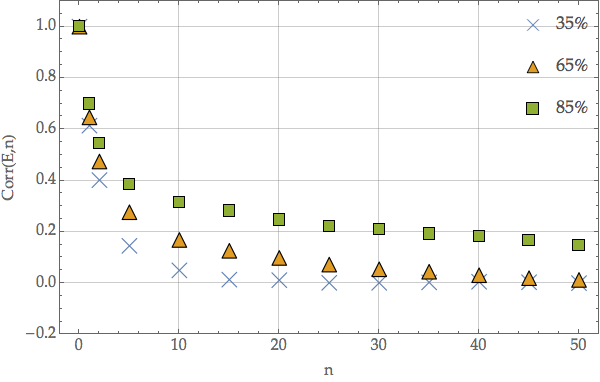
\includegraphics[width=\textwidth]{Figures/MCEnergyCorrelations}
	\caption[MC: Energy Correlation Series]{Energy correlation for a $4\times10^4$ equilibrated sample at $T=0.5$ and $\rho=0.35$. According to the acceptance ratio, the correlation length differs.}
	\label{fig:MCCorrSeries}
\end{figure}\\
To use nearly uncorrelated data for a meaningful quantity of interest with this setting, a sample distance of approximately $50$ MC-Steps is sufficient.
For the final estimate, the quantity with errors then resolves to
\begin{align}
	\begin{split}
	  \begin{array}{l l}
	  \overline{E}&=\hspace{0.2cm}\frac{1}{N}\sum\limits_{i=1}^N E_i\smallskip\\
	  	\Delta \overline{E}&=\hspace{0.2cm}\sqrt{\frac{1}{N-1}\sum\limits_{j=1}^{N}(\overline{E}-E_j)^2}
	  \end{array}
	  \hspace{1cm}\Braket{E} &=\overline{E} \pm \frac{\Delta E}{\sqrt N}.
	\end{split}
\end{align}
\medskip\\
In order to gain reasonable correlation trends, the samples have to be re\-corded in equilibrated states.
The time, until such a step is reached, depends on the temperature and density of the system - near the critical point of the phase diagramme, the convergence behaviour is worse than apart~(see Fig.~\ref{fig:MCEnergyConvergence}).
\begin{figure}[ht]
	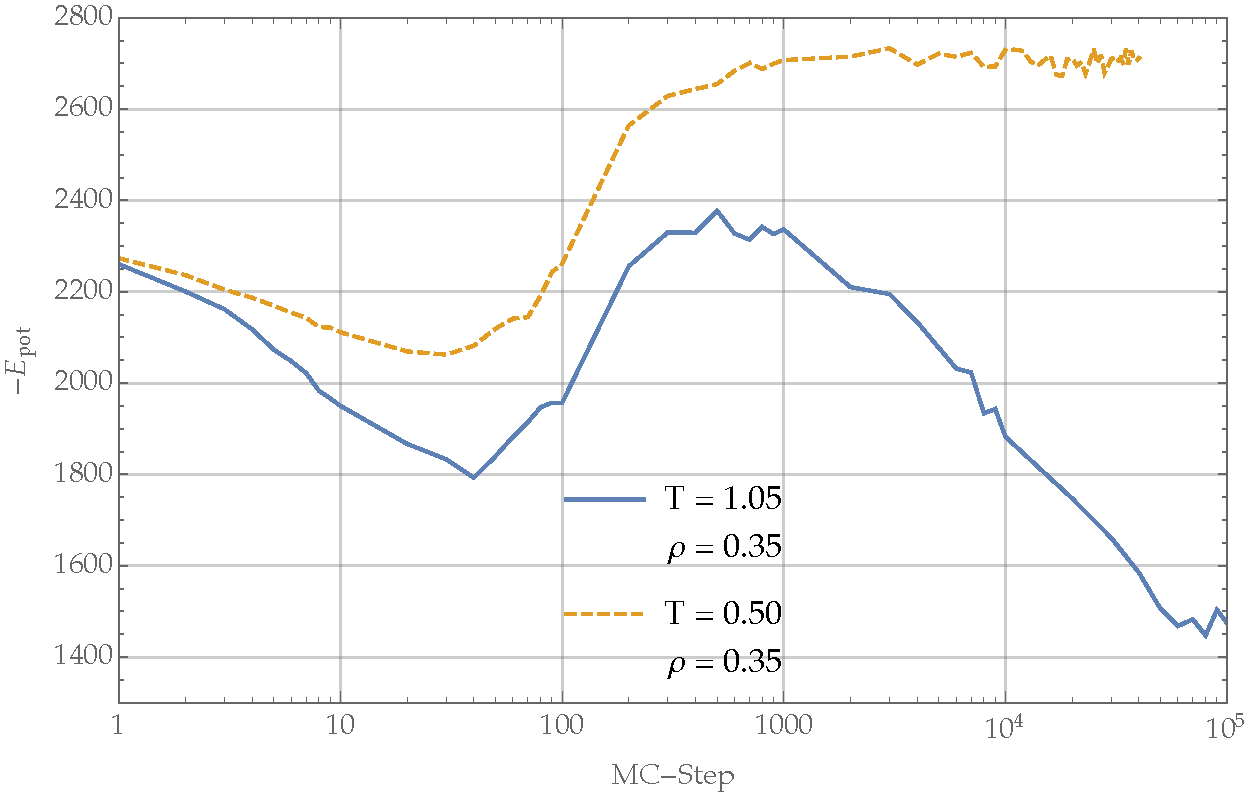
\includegraphics[width=\textwidth]{Figures/MCEnergyConvergence.pdf}
	\caption[MC: Energy Convergence Behaviour]{Energy convergence behaviour apart and near the critical point.}
	\label{fig:MCEnergyConvergence}
\end{figure}\\
Hence one has to analyse the correlation and convergence for each measurement in particular and decide which parameters are best, but due to time frame limitations, the setting is fixed and listed in Tab.~\ref{tbl:MCSettings}.
\begin{table}[ht]
	\centering
	\begin{tabular}{l | l}
		System specifics &Setting \\
		\hline
		Number of particles &chosen according to density and system size\\
		Acceptance ratio&roughly set $\approx$ \SI{60}{\percent}\\
		Equilibration&after $2\times10^5$ MC-Steps\\
		Quantity series&$6\times10^3$ samples with $150$ MC-Steps distance\\
	\end{tabular}
	\caption[MC: Settings]{Listing with settings for the measurement via Monte-Carlo.}
	\label{tbl:MCSettings}
\end{table}\\
The same considerations have been made in case for Molecular Dynamics, but the thermostat requires extra mentioning.
